% !TeX TS-program = xelatex

\documentclass{beamer}
%Set the slide theme
%Change to meet your taste
% Madrid, Copenhagen, Berlin, ... works
\usetheme{metropolis}


\usepackage{xecolor}
\usepackage{amsmath}
%\usefonttheme[onlymath]{serif} %Change the math font

\usepackage{xepersian}
\settextfont[Path=fonts/]{Parastoo}

%---------------------------------------------------------------------------------
% Seetings to force Beamer works with Xepersian and RTL typesetting
%-------------------------------------------------------------------------------
%\raggedleft

% For right to left lists (itemize and enumerate)
\makeatletter
\newcommand{\RTList}{\raggedleft\rightskip\@totalleftmargin}
\makeatother
% Correct the bullet for RTL texts
\setbeamertemplate{itemize item}{\scriptsize\raise1.25pt%
 \hbox{\donotcoloroutermaths$\blacktriangleleft$}} 

% To force beamer use numbering in captions
\setbeamertemplate{caption}[numbered]{}% Number float-like environments



%---------------------------------------------------------------------------------
\title{
	عنوان پروژه
}
\subtitle{}
\author{پرهام الوانی}
\institute{دانشکده مهندسی کامپیوتر و فناوری اطلاعات}
\date{پاییز ۱۳۹۶}

\begin{document}
\begin{persian}
%------------------------------------------
% Title page
%------------------------------------------
\begin{frame}
\maketitle
\end{frame}

% To adjust the paragraphs in RTL
\everypar{\rightskip\rightmargin}
%-------------------------------------------------------------------------------
\begin{frame}{طرح مساله}
	\begin{itemize}\RTList
		\item سمت کاربر
		\item سمت دیتاسنتر
		\begin{itemize}\RTList
			\item \lr{ETSI GS MANO}
		\end{itemize}
	\end{itemize}
\end{frame}
\begin{frame}{مساله اول}
	\par
	\lr{NFVO} وظیفه‌ی استقرار زنجیره‌های کارکرد سرویس را برعهده دارد.
	همانگونه که در مستند \lr{ETSI} نیز آمده است هر نمونه از کارکردهای مجازی شبکه نیاز دارد
	تحت مدیریت یکی از \lr{VNFM}های موجود در شبکه باشد.
\end{frame}
\begin{frame}
	\begin{center}\begin{figure}
		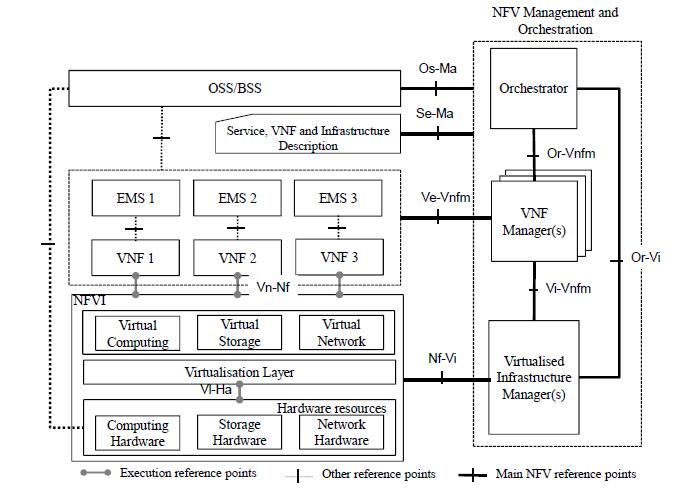
\includegraphics[scale=0.4]{images/nfv-arch.jpg}
		\caption{معماری سطح بالای مجازی‌سازی کارکردهای شبکه}
	\end{figure}\end{center}
\end{frame}
\begin{frame}
	\par
	یکی از وظایف \lr{VNFM} مانیتور کردن وضعیت و خطاهای نمونه‌ها می‌باشد
	این امر باعث افزایش بار پردازشی \lr{VNFM} می‌گردد
	و از سوی دیگر تحلیل این اطلاعات می‌بایست با تاخیر معقولی صورت پذیرد که این امر
	نیاز به یک بستر ارتباطی مطمئن دارد.
\end{frame}
\begin{frame}
	\par
	پذیرفتن بیشترین تقاضای زنجیره‌ کارکرد سرویس با در نظر گرفتن نیاز هر نمونه کارکرد مجازی شبکه به یک \lr{VNFM}.
\end{frame}
\begin{frame}
	\begin{itemize}\RTList
		\item n تقاضای زنجیره‌ کارکرد سرویس به صورت کامل داریم.
		\item نمونه‌ها بین زنجیره‌ها به اشتراک گذاشته نمی‌شوند.
	\end{itemize}
\end{frame}

\end{persian}
\end{document}